\appendix
\chapter{Functional Analysis}
\begin{figure}[H]
	\centering
	\subfloat[Cell components]{
		\includegraphics[width=\textwidth]{asymmetry/FUMA gene2func/joinedDatasets/mean_imputed/not_subsampled/partitionsSummary/GO_CC.pdf}
	}
	\quad
	\subfloat[Biological processes]{
		\includegraphics[width=\textwidth]{asymmetry/FUMA gene2func/joinedDatasets/mean_imputed/not_subsampled/partitionsSummary/GO_BP.pdf}
	}
	\quad
	\subfloat[Molecular function]{
		\includegraphics[width=\textwidth]{asymmetry/FUMA gene2func/joinedDatasets/mean_imputed/not_subsampled/partitionsSummary/GO_MF.pdf}
	}
	\caption[GO terms enrichment analysis]{\Ac{go} terms enrichment analysis -log10 P-values (the higher value and the darker color, the more significant), as computed by FUMA, with the gene set augmented by GREAT.For all three cases, the entire hemisphere and the four 2nd level partition were assessed, however not all of the tests displayed a significant signal with \ac{go} terms.}
	\label{fig:go}
\end{figure}
\begin{figure}[H]
	\centering
	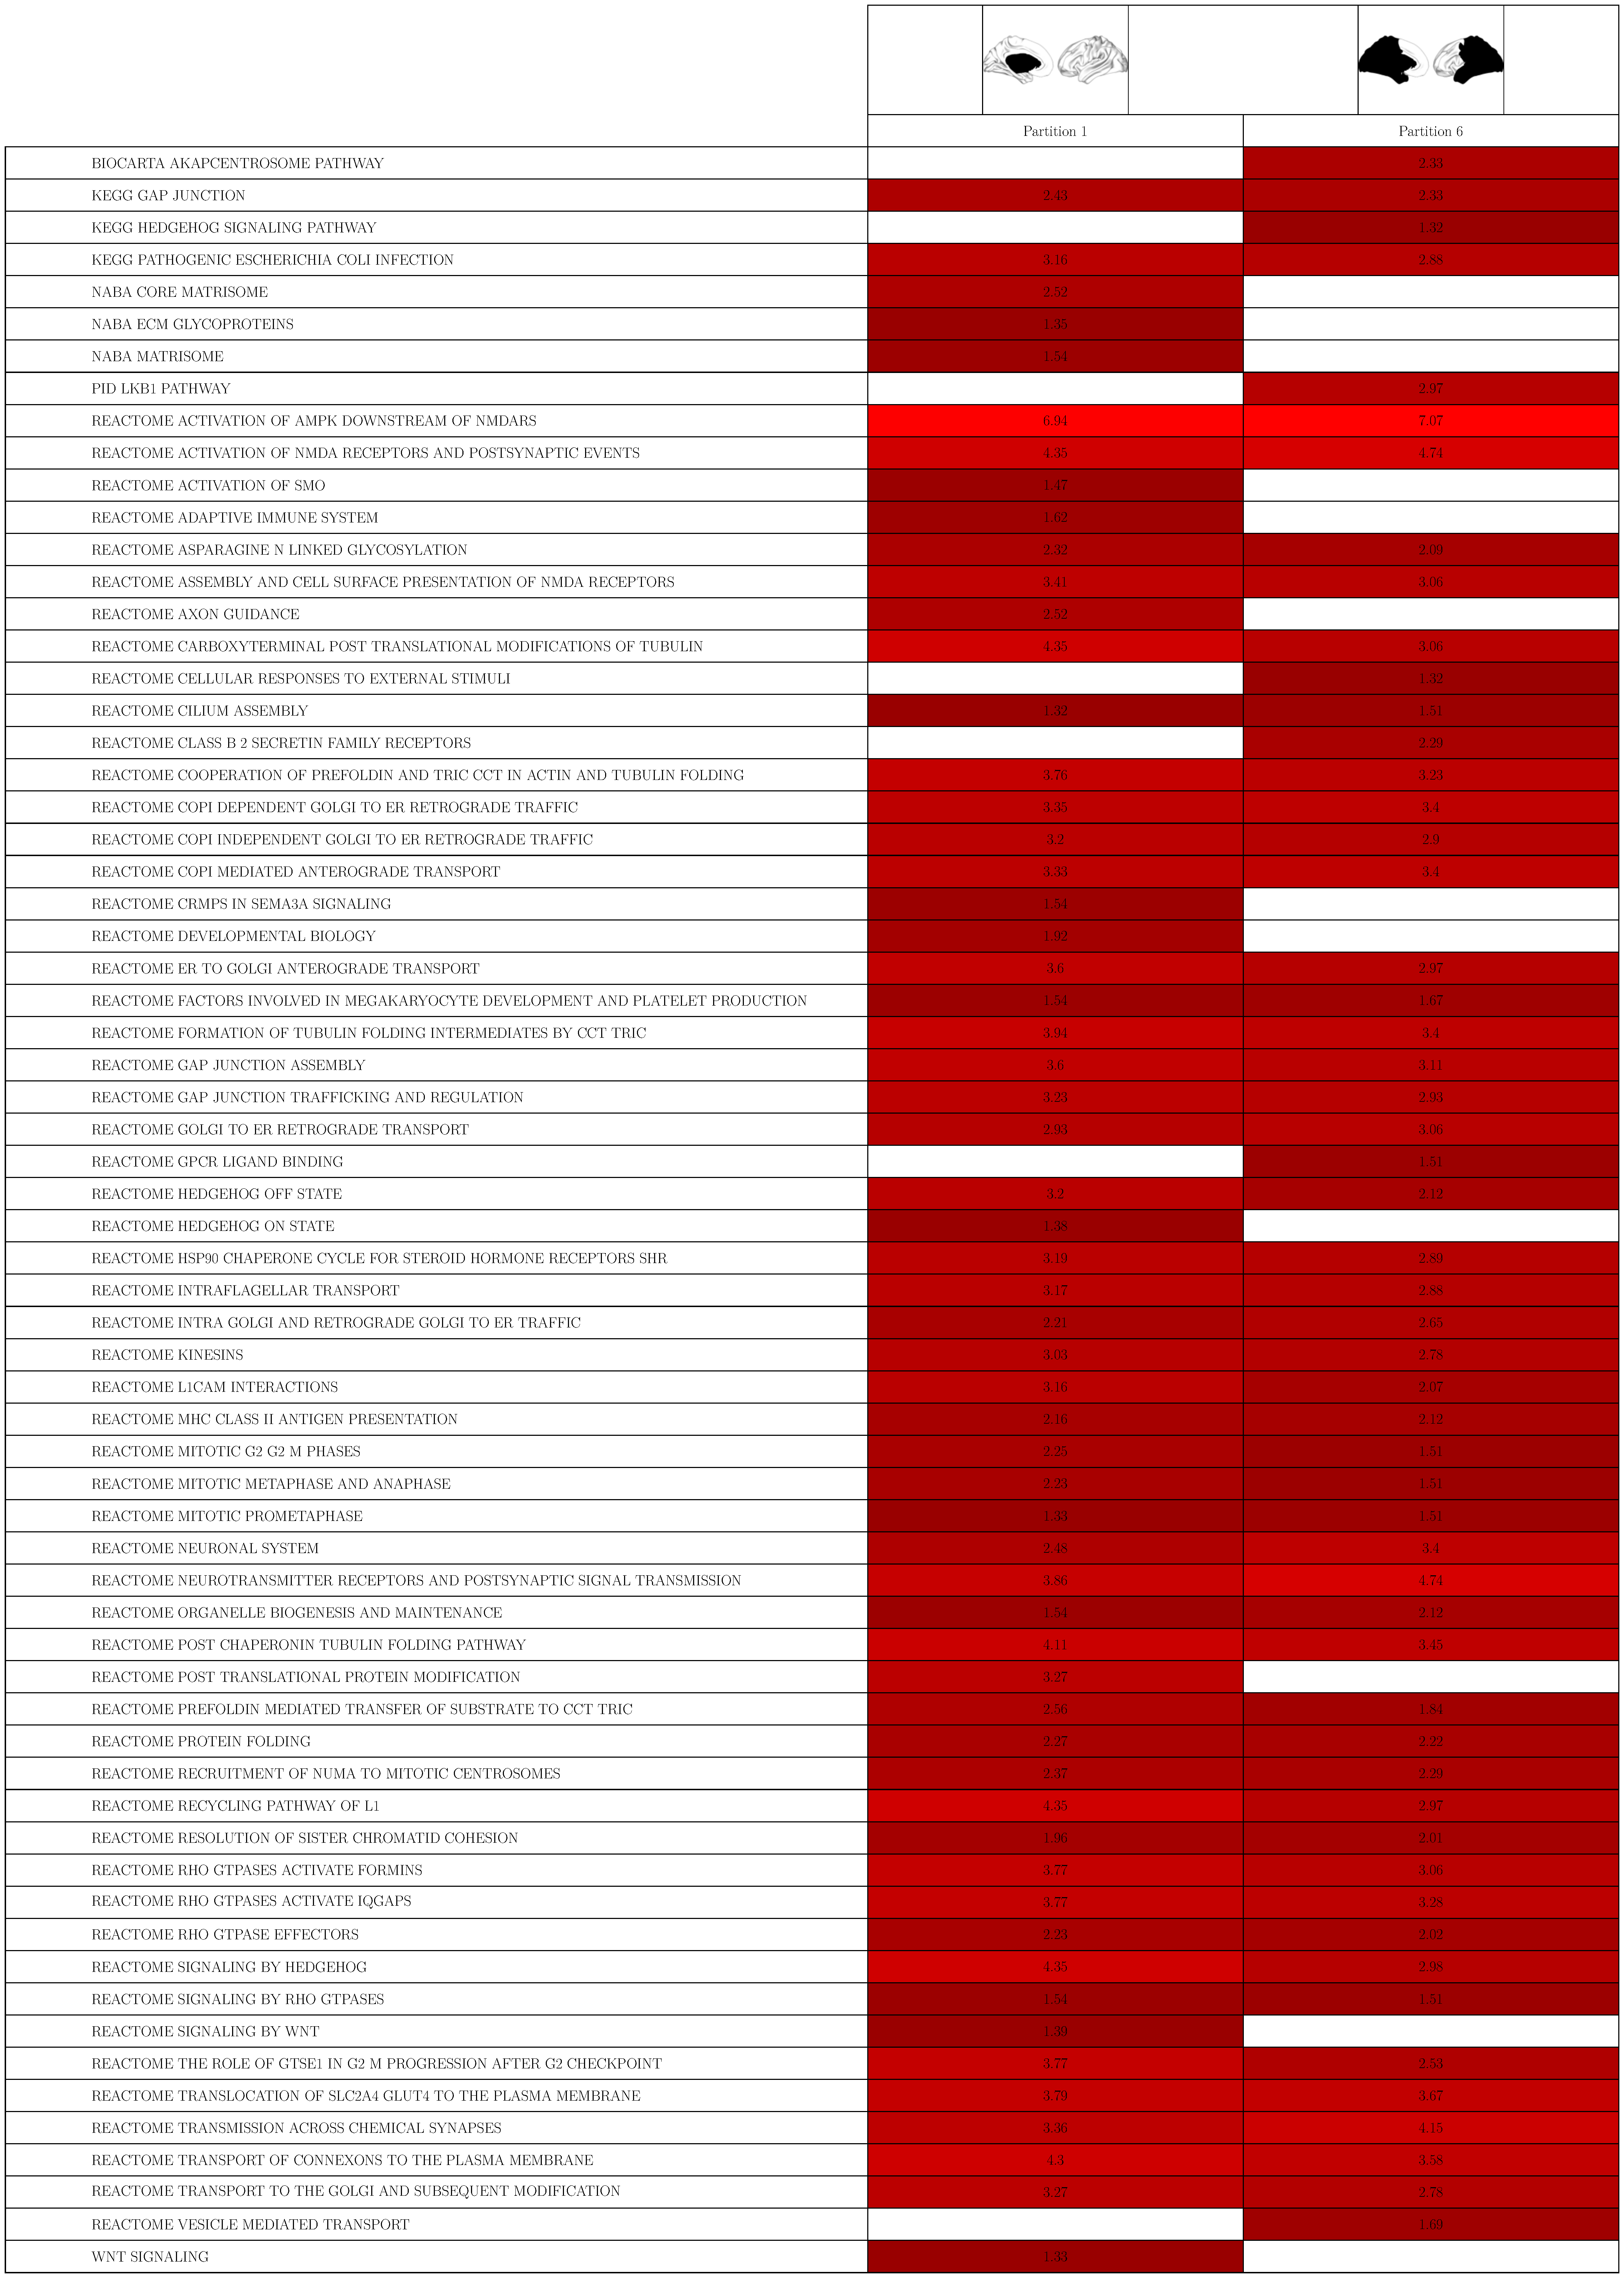
\includegraphics[width=\textwidth]{asymmetry/FUMA gene2func/joinedDatasets/mean_imputed/not_subsampled/partitionsSummary/canonical_pathways.pdf}
	
	\caption[Canonical pathways gene set enrichment analysis]{Differential gene set enrichment analysis performed on various canonical pathways reported by KEGG and Reactome, as computed by FUMA. Displayed -log10 P-values have increased lightness the higher the value.}
	\label{fig:can_pathways}
\end{figure}
\begin{figure}[H]
	\centering
	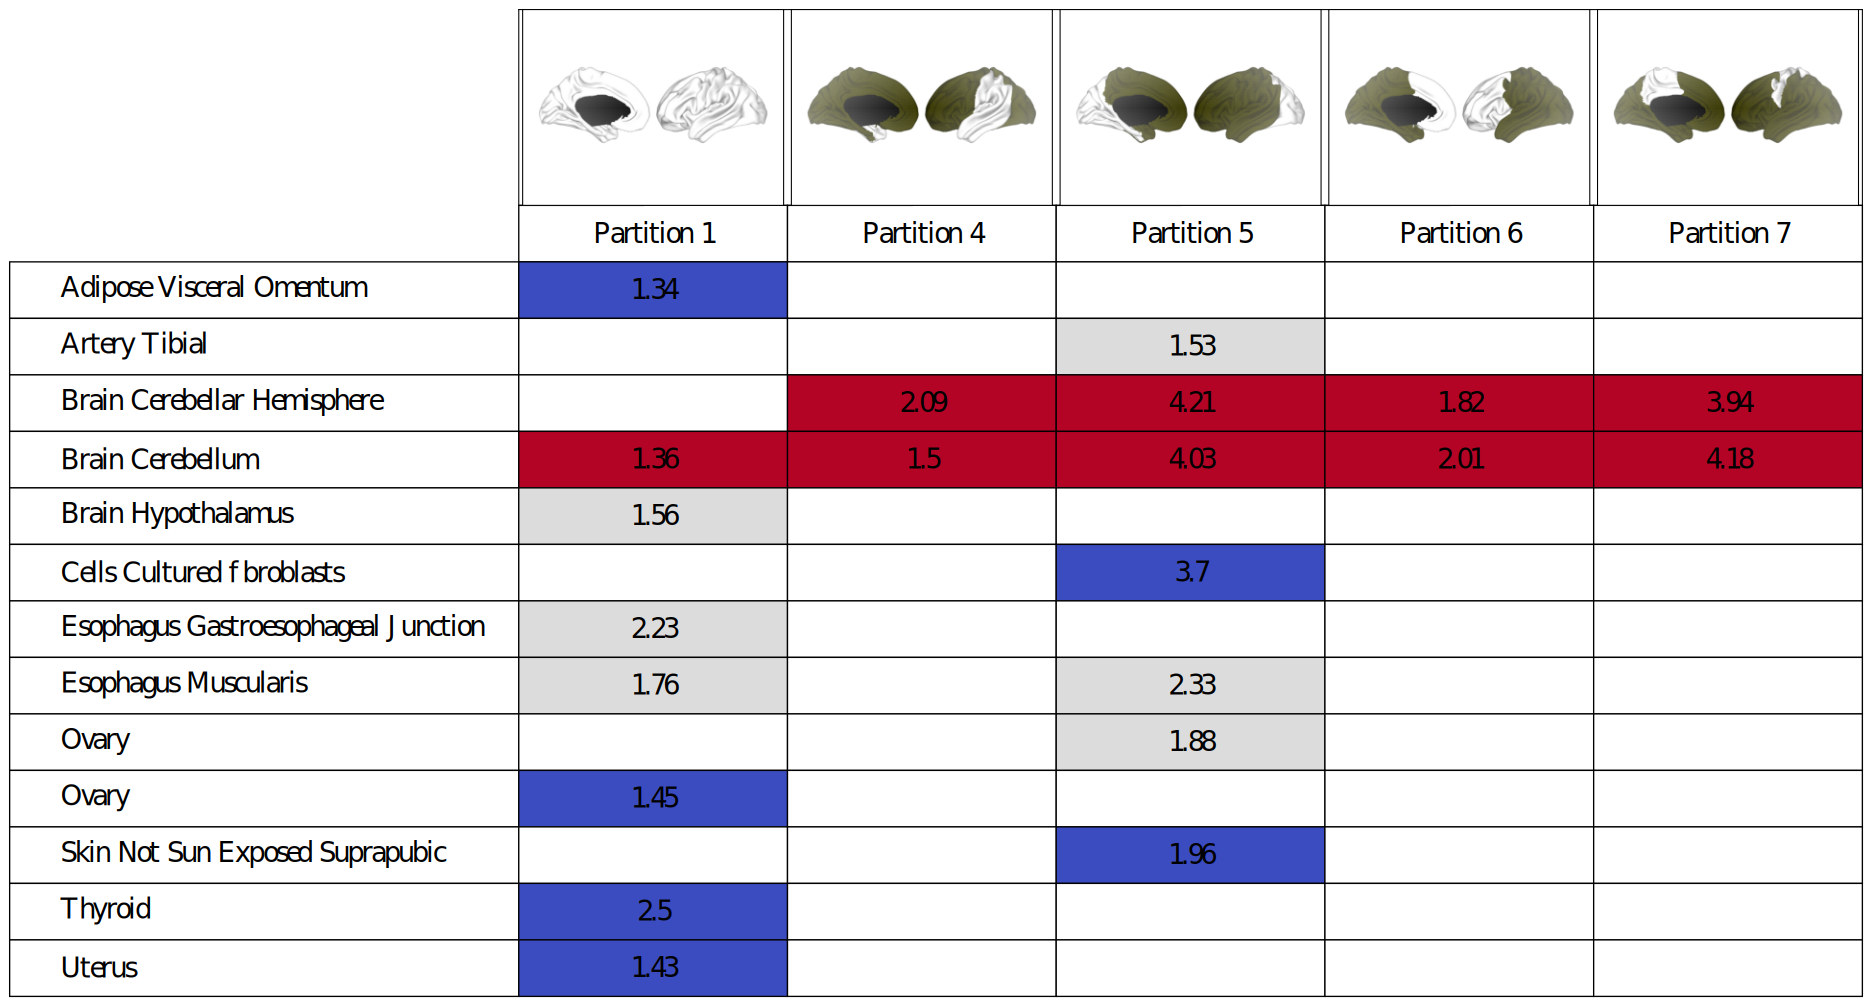
\includegraphics[width=\textwidth]{asymmetry/FUMA gene2func/joinedDatasets/mean_imputed/not_subsampled/partitionsSummary/DEG.pdf}
	
	\caption[Differential gene expression enrichment analysis]{Differential gene expression enrichment analysis performed on different tissues. Displayed -log10 P-values, as computed by FUMA using the identified partition-specific gene sets, are displayed in blue if the relation favors downregulated genes, red if it favors upregulated ones, or gray, if both downregulated and upregulated gene subsets are significantly enriched.}
	\label{fig:de_genes}
\end{figure}
\begin{figure}[H]
	\centering
	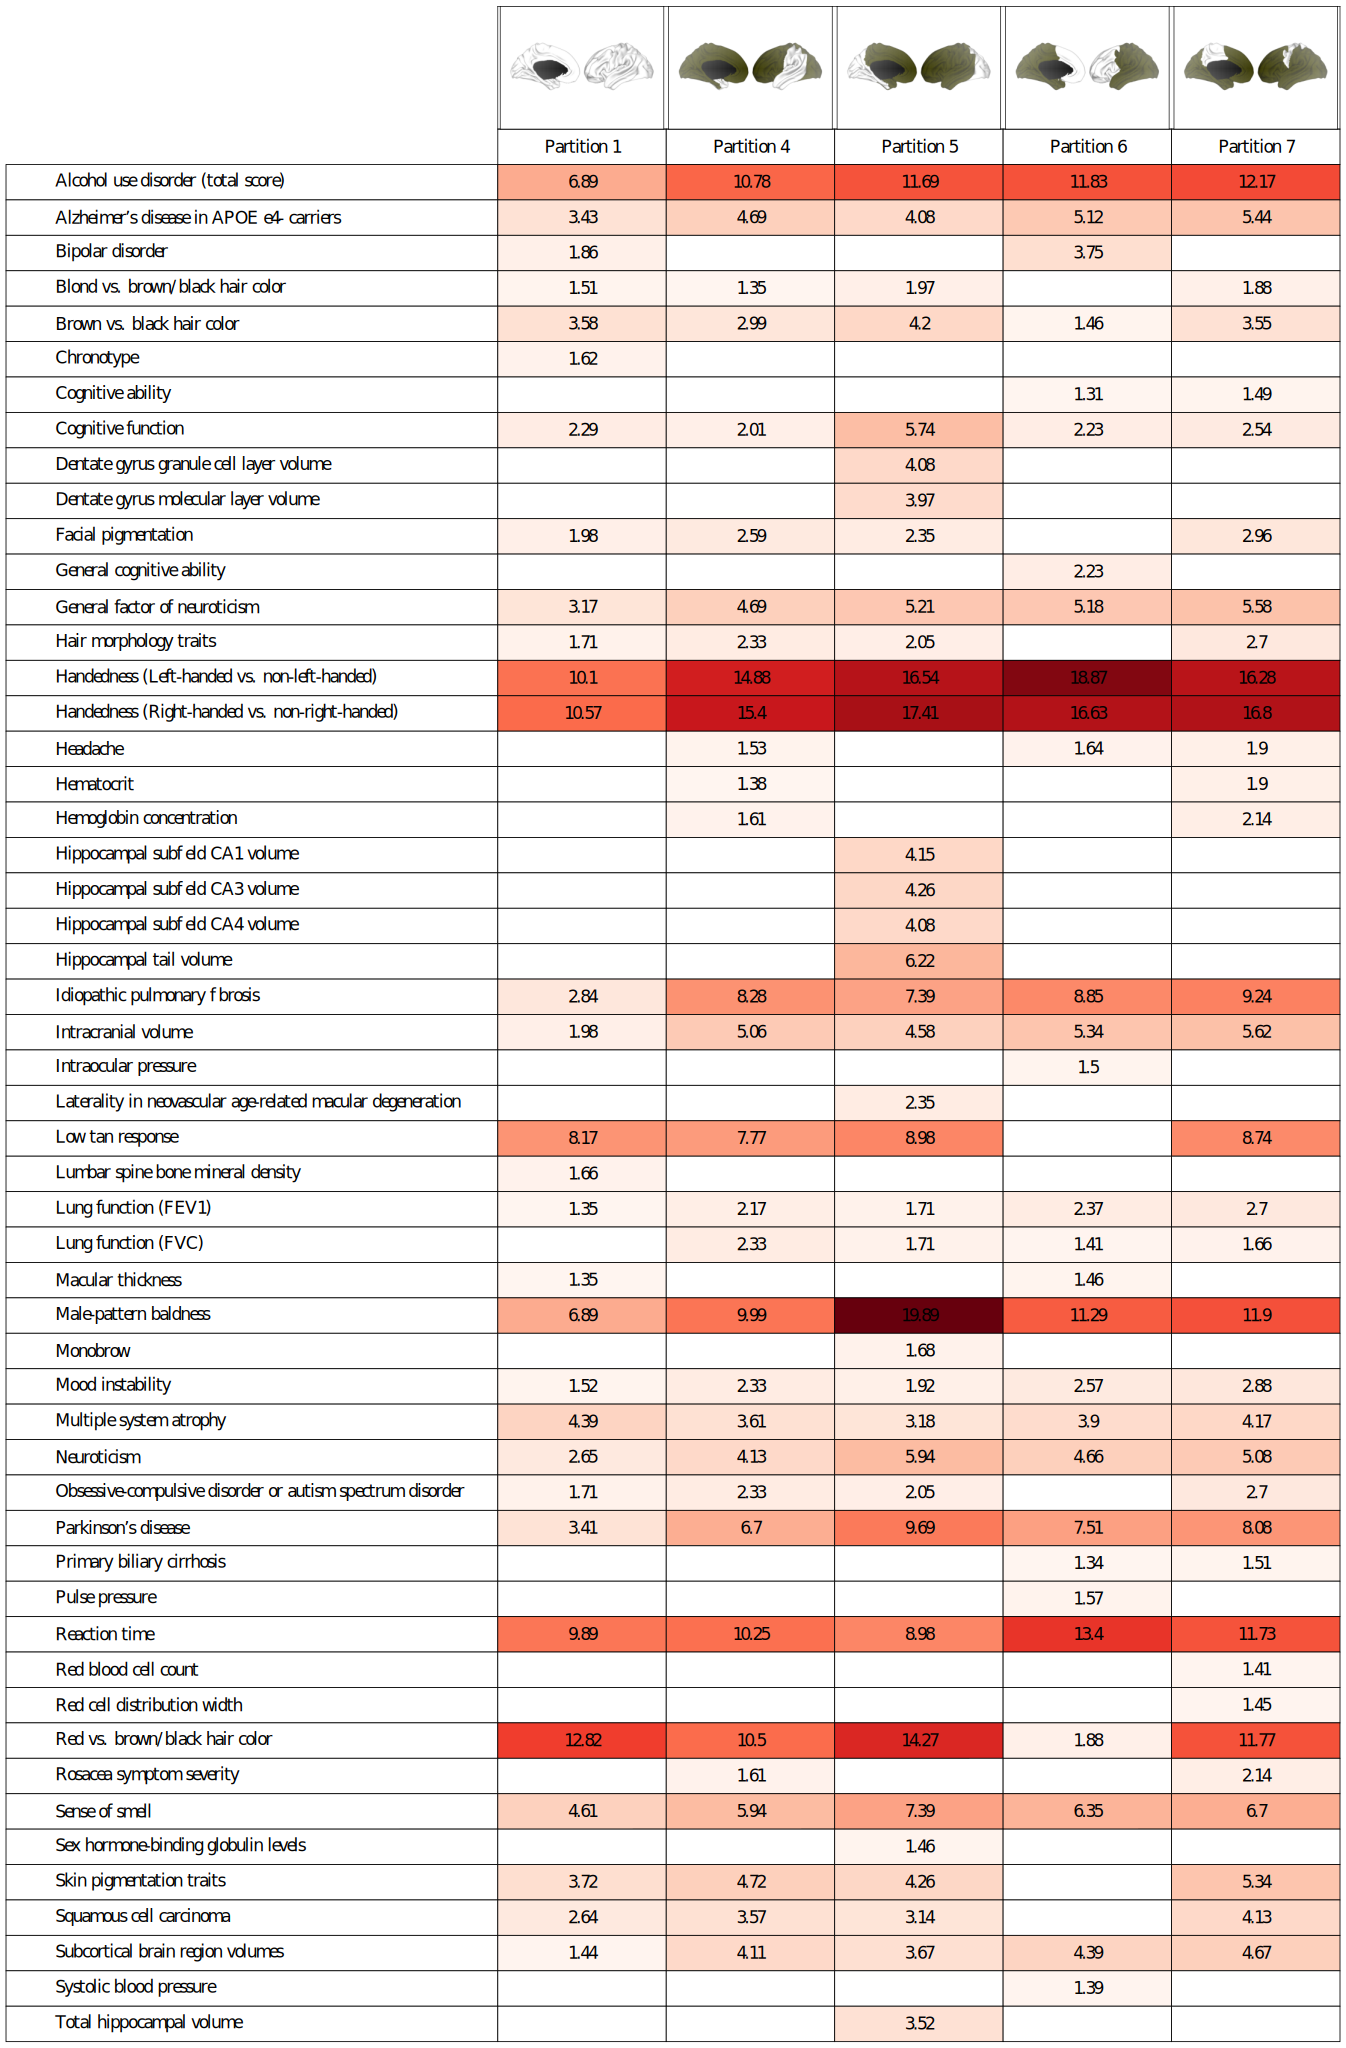
\includegraphics[width=\textwidth]{asymmetry/FUMA gene2func/joinedDatasets/mean_imputed/not_subsampled/partitionsSummary/GWASCatalog.pdf}
	
	\caption[GWAS Catalog gene set enrichment analysis]{Differential gene set enrichment analysis performed on various traits reported by GWAS catalog, as computed by FUMA. -log10 P-values are shown, with increased lightness the higher the value.}
	\label{fig:gw_catalog}
\end{figure}
